
\documentclass{document}
\usepackage[backend=biber,style=gb7714-2015]{biblatex} % cqu毕设论文引用格式,国标
\addbibresource{assets/bib/references.bib} % 加载参考文献数据库


\begin{document}
\makecovercn
  {毕业设计题目}
  {学生姓名}
  {学号}
  {指导教师}
  {}%助理老师(选填)
  {专业}
  {}%原学校(选填)
  {2025}

\makecoveren
  {XXX Computational Model}
  {WANG Jianhua}
  {Prof. YANG XX}
  {} %第二个导师(选填)
  {Intelligent Connected Vehicle}
  {Intelligent Manufacturing}%第二个专业(选填)
  {} %原学校(选填)
  {2025} 


\addcontentsline{toc}{section}{摘要}  
\begin{cquabstract}
%空一行会自动换自然段,一段文字后使用\\会换行但没有段首缩进

摘要是论文(设计)内容不加注释和评论的简短陈述,应以第三人称陈述。它应独立性和自含性,即不阅读论文(设计)的全文,就能获得必要的信息。\\

摘要一般应说明研究工作的目的和意义、研究思想和方法、研究过程、研究结果和最终结论等。摘要中一般不用图、表、化学结构式、计算机程序,不用非公知公用的符号、术语和非法定的计量单位。

摘要页置于英文题名页后。 
中文摘要一般为300~400字,用宋体小四号。 \\
关键词是指从论文(设计)的标题、摘要、正文中抽取的对表达论文(设计)主题起关键作用,且具有检索意义的词语。关键词应体现论文(设计)特色,具有语义性,在论文(设计)中有明确的出处。一般每篇论文(设计)应选取3-5个词作为关键词,以显著的字符另起一行,排在同种语言摘要的下方,尽量用《汉语主题词表》或各专业主题词表提供的规范词。\\
\end{cquabstract}
  
\begin{cqukeywords}%中文分号
    XXXX;XXXX;XXXX
\end{cqukeywords}

\addcontentsline{toc}{section}{ABSTRACT}  
  % 英文摘要
\begin{cquabstracten}
  The abstract is a concise statement of the content of the thesis (design) without annotations or comments. It should be compact and refined.
\end{cquabstracten}

% 英文关键词
\begin{cqukeywordsen}
  XXXX; XXXX; XXXX
\end{cqukeywordsen}
  
\begin{cqucontents}

\end{cqucontents}



%下面就是正文了
\pagestyle{essaystyle}
\pagenumbering{arabic} % 页码为阿拉伯数字


\section{研究背景}
研究背景部分需要详细说明研究的动机和相关领域的现状。

\subsection{国内外研究现状}
国内外研究现状部分需要总结已有的研究成果,并指出研究的不足。

\subsubsection{国内研究现状}
国内研究现状部分需要重点分析国内的研究进展。

\subsubsection{国外研究现状}
国外研究现状部分需要重点分析国外的研究进展。

\section{研究意义}
研究意义部分需要说明本研究的创新点和实际应用价值。
摘要是论文(设计)内容不加注释和评论的简短陈述,应以第三人称陈述。它应具有独立性和自含性,即不阅读论文(设计)的全文,就能获得必要的信息。
摘要一般应说明研究工作的目的和意义、研究思想和方法、研究过程、研究结果和最终结论等。摘要中一般不用图、表、化学结构式、计算机程序,不用非公知公用的符号、术语和非法定的计量单位。\cite{YXXY20250307001}
摘要页置于英文题名页后。 
中文摘要一般为300~400字,用宋体小四号。

\begin{figure}[htbp]
    \centering
    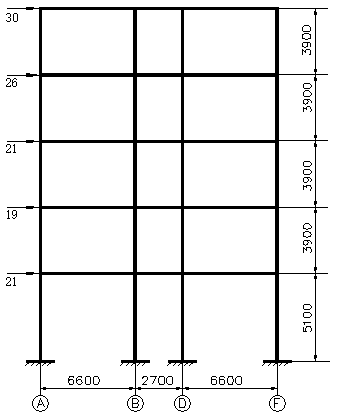
\includegraphics[width=0.4\textwidth]{assets/images/image.png}
    \caption{模型示意图}
    \label{fig:model}%可加可不加
\end{figure}

关键词是指从论文(设计)的标题、摘要、正文中抽取的对表达论文(设计)主题起关键作用,且具有检索意义的词语。关键词应体现论文(设计)特色,具有语义性,在论文(设计)中有明确的出处。一般每篇论文(设计)应选取3-5个词作为关键词,以显著的字符另起一行,排在同种语言摘要的下方,尽量用《汉语主题词表》或各专业主题词表提供的规范词。\cite{10.1145/3583780.3615277}  

\section{理论分析}

\subsection{模型建立}

如图所示,建立了一个简化的模型来分析结构的受力情况。模型中考虑了主要的荷载和边界条件。



对对对

\subsubsection{模型dada}
根据《荷载规范》,本工程上屋面活荷载取值为 $q_w = 1.5 \, \text{kN/m}^2$。

%表格模板,可以参考一下,个人latex的表格非常方便而且好更改
\begin{table}[htbp]
    \centering
    \caption{左风作用下简截计算}
    \begin{tabular}{cccccc}
      \toprule
      层次 & $Z(m)$ & $\mu$ & $\beta$ & $q_w (\text{kN/m}^2)$ & $W (\text{kN})$ \\
      \midrule
      1 & 4.5 & … & … & … & … \\
      2 & … & … & … & … & … \\
      \bottomrule
    \end{tabular}
\end{table}
\subsection{实验设计}
摘要是论文(设计)内容不加注释和评论的简短陈述,应以第三人称陈述。它应具有独立性和自含性,即不阅读论文(设计)的全文,就能获得必要的信息。
摘要一般应说明研究工作的目的和意义、研究思想和方法、研究过程、研究结果和最终结论等。摘要中一般不用图、表、化学结构式、计算机程序,不用非公知公用的符号、术语和非法定的计量单位。
摘要页置于英文题名页后。   git add

中文摘要一般为300~400字,用宋体小四号。 
关键词是指从论文(设计)的标题、摘要、正文中抽取的对表达论文(设计)主题起关键作用,且具有检索意义的词语。关键词应体现论文(设计)特色,具有语义性,在论文(设计)中有明确的出处。一般每篇论文(设计)应选取3-5个词作为关键词,以显著的字符另起一行,排在同种语言摘要的下方,尽量用《汉语主题词表》或各专业主题词表提供的规范词


% 引用文献\cite{key2023}
\clearpage
% \pagestyle{essaystyle}
\addcontentsline{toc}{section}{参考文献}  
\printbibliography




\begin{cquappendix}{A: 公式推导}
    % \pagestyle{appendixstyle}
    XX公式的推导过程是:
    
    中文宋体五号,英文 Times New Roman 五号,行距固定值 20 磅,字数不少于 3000 字。
    
    以下内容包括在附录中:
    \begin{enumerate}
        \item 正文中过长的公式推导与证明过程可以在附录中依次给出;
        \item 与正文紧密相关的作者自己的分析、证明及工具用表格(如调查问卷)等;
        \item 在正文中无法列出的实验数据、程序等;
        \item 设计或论文使用的缩写及程序说明等;
        \item 学生在读期间参加的科研项目或科研训练项目、发表的论文、取得的其他科研成果等。
    \end{enumerate}

    \begin{enumerate}
        \item 正文中过长的公式推导与证明过程可以在附录中依次给出;
        \item 与正文紧密相关的作者自己的分析、证明及工具用表格(如调查问卷)等;
        \item 在正文中无法列出的实验数据、程序等;
        \item 设计或论文使用的缩写及程序说明等;
        \item 学生在读期间参加的科研项目或科研训练项目、发表的论文、取得的其他科研成果等。
    \end{enumerate}

    \begin{enumerate}
        \item 正文中过长的公式推导与证明过程可以在附录中依次给出;
        \item 与正文紧密相关的作者自己的分析、证明及工具用表格(如调查问卷)等;
        \item 在正文中无法列出的实验数据、程序等;
        \item 设计或论文使用的缩写及程序说明等;
        \item 学生在读期间参加的科研项目或科研训练项目、发表的论文、取得的其他科研成果等。
    \end{enumerate}

    \begin{enumerate}
        \item 正文中过长的公式推导与证明过程可以在附录中依次给出;
        \item 与正文紧密相关的作者自己的分析、证明及工具用表格(如调查问卷)等;
        \item 在正文中无法列出的实验数据、程序等;
        \item 设计或论文使用的缩写及程序说明等;
        \item 学生在读期间参加的科研项目或科研训练项目、发表的论文、取得的其他科研成果等。
    \end{enumerate}

    \begin{enumerate}
        \item 正文中过长的公式推导与证明过程可以在附录中依次给出;
        \item 与正文紧密相关的作者自己的分析、证明及工具用表格(如调查问卷)等;
        \item 在正文中无法列出的实验数据、程序等;
        \item 设计或论文使用的缩写及程序说明等;
        \item 学生在读期间参加的科研项目或科研训练项目、发表的论文、取得的其他科研成果等。
    \end{enumerate}

    \begin{enumerate}
        \item 正文中过长的公式推导与证明过程可以在附录中依次给出;
        \item 与正文紧密相关的作者自己的分析、证明及工具用表格(如调查问卷)等;
        \item 在正文中无法列出的实验数据、程序等;
        \item 设计或论文使用的缩写及程序说明等;
        \item 学生在读期间参加的科研项目或科研训练项目、发表的论文、取得的其他科研成果等。
    \end{enumerate}

    \begin{enumerate}
        \item 正文中过长的公式推导与证明过程可以在附录中依次给出;
        \item 与正文紧密相关的作者自己的分析、证明及工具用表格(如调查问卷)等;
        \item 在正文中无法列出的实验数据、程序等;
        \item 设计或论文使用的缩写及程序说明等;
        \item 学生在读期间参加的科研项目或科研训练项目、发表的论文、取得的其他科研成果等。
    \end{enumerate}

    \begin{enumerate}
        \item 正文中过长的公式推导与证明过程可以在附录中依次给出;
        \item 与正文紧密相关的作者自己的分析、证明及工具用表格(如调查问卷)等;
        \item 在正文中无法列出的实验数据、程序等;
        \item 设计或论文使用的缩写及程序说明等;
        \item 学生在读期间参加的科研项目或科研训练项目、发表的论文、取得的其他科研成果等。
    \end{enumerate}

    \begin{enumerate}
        \item 正文中过长的公式推导与证明过程可以在附录中依次给出;
        \item 与正文紧密相关的作者自己的分析、证明及工具用表格(如调查问卷)等;
        \item 在正文中无法列出的实验数据、程序等;
        \item 设计或论文使用的缩写及程序说明等;
        \item 学生在读期间参加的科研项目或科研训练项目、发表的论文、取得的其他科研成果等。
    \end{enumerate}

    \begin{enumerate}
        \item 正文中过长的公式推导与证明过程可以在附录中依次给出;
        \item 与正文紧密相关的作者自己的分析、证明及工具用表格(如调查问卷)等;
        \item 在正文中无法列出的实验数据、程序等;
        \item 设计或论文使用的缩写及程序说明等;
        \item 学生在读期间参加的科研项目或科研训练项目、发表的论文、取得的其他科研成果等。
    \end{enumerate}
\end{cquappendix}

\begin{cquappendix}{B: 程序代码}
    
    以下是程序代码的呈现示例:
    
    \begin{lstlisting}[language=Python, caption={Python 示例代码}]
    def factorial(n):
        if n == 0:
            return 1
        else:
            return n * factorial(n-1)
    \end{lstlisting}
    
\end{cquappendix}

\begin{cquacknowledgements}
    

    致谢部分需要感谢指导教师、同学和家人等对研究的支持和帮助。\\
        
   
           感谢指导教师的悉心指\\
           感谢同学们的支持与帮助;\\
            感谢家人的理解与支持。\\
            感谢指导教师的悉心指\\
            感谢同学们的支持与帮助;\\
             感谢家人的理解与支持。\\
             感谢指导教师的悉心指\\
             感谢同学们的支持与帮助;\\
              感谢家人的理解与支持。\\
              感谢指导教师的悉心指\\
              感谢同学们的支持与帮助;\\
               感谢家人的理解与支持。\\
               感谢指导教师的悉心指\\
               感谢同学们的支持与帮助;\\
                感谢家人的理解与支持。\\
                感谢指导教师的悉心指\\
                感谢同学们的支持与帮助;\\
                 感谢家人的理解与支持。\\
                 感谢指导教师的悉心指\\
                 感谢同学们的支持与帮助;\\
                  感谢家人的理解与支持。\\
                  感谢指导教师的悉心指\\
                  感谢同学们的支持与帮助;\\
                   感谢家人的理解与支持。\\
                   感谢指导教师的悉心指\\
                   感谢同学们的支持与帮助;\\
                    感谢家人的理解与支持。\\
                    感谢指导教师的悉心指\\
                    感谢同学们的支持与帮助;\\
                     感谢家人的理解与支持。\\
                     感谢指导教师的悉心指\\
                     感谢同学们的支持与帮助;\\
                      感谢家人的理解与支持。\\
                      感谢指导教师的悉心指\\
                      感谢同学们的支持与帮助;\\
                       感谢家人的理解与支持。\\
                       感谢指导教师的悉心指\\
                       感谢同学们的支持与帮助;\\
                        感谢家人的理解与支持。\\
                        感谢指导教师的悉心指\\
                        感谢同学们的支持与帮助;\\
                         感谢家人的理解与支持。\\
                         感谢指导教师的悉心指\\
                         感谢同学们的支持与帮助;\\
                          感谢家人的理解与支持。\\
                          感谢指导教师的悉心指\\
                          感谢同学们的支持与帮助;\\
                           感谢家人的理解与支持。\\
                           感谢指导教师的悉心指\\
                           感谢同学们的支持与帮助;\\
                            感谢家人的理解与支持。\\
                            感谢指导教师的悉心指\\
                            感谢同学们的支持与帮助;\\
                             感谢家人的理解与支持。\\
                             感谢指导教师的悉心指\\
                             感谢同学们的支持与帮助;\\
                              感谢家人的理解与支持。\\
                              感谢指导教师的悉心指\\
                              感谢同学们的支持与帮助;\\

\end{cquacknowledgements}

\end{document}